
\setlength{\epigraphwidth}{0.75\textwidth}
\epigraph{\textit{"Learning from interaction is a foundational idea underlying nearly all theories of learning and intelligence"}}{--Rich Sutton and Andrew Barto, \textit{Reinforcement Learning: An Introduction}}


\section{Introduction}
\subsection{Autonomous Navigation and Control via Reinforcement Learning}

\begin{wrapfigure}{r}{0.45\textwidth}
    \centering
    \vspace{-15pt}
    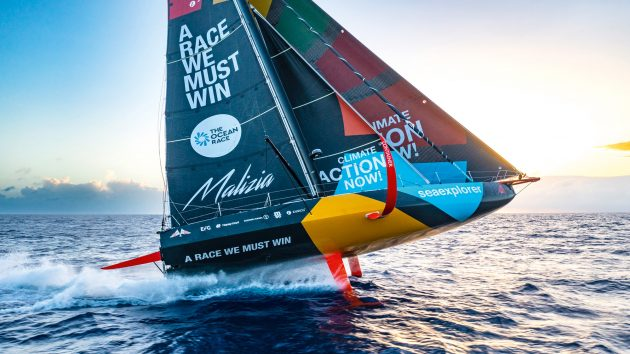
\includegraphics[width=0.42\textwidth]{resources/img/chapter1/boat.png}
    \caption{The IMOCA 60 \emph{Malizia Seaexplorer}, one of the world's fastest monohulls.}
    \label{fig:imoca}
    \vspace{-17pt}
\end{wrapfigure}
The application of Deep Reinforcement Learning (DRL) in autonomous navigation and control is becoming increasingly ubiquitous. In the context of autonomous sailing, DRL addresses a high dimensional optimal control problem characterized by nonlinear dynamics and significant environmental uncertainties. The ability of a DRL agent to learn this control problem directly correlates with performance improvements in elite competitive environments, such as the solo round the world Vendée Globe\footnote{The Vendée Globe is a non stop, round the world yacht race widely regarded as one of the most demanding sailing competitions.}. Racing environments often employ a specialized class of vessel known as a \emph{sailboat}. Compared to traditional motorized vessels sailboats operate without an engine and they rely entirely on wind as their primary power source. Nevertheless, modern racing sailboats are equipped with sophisticated autopilot systems that are essential for both sailor safety and competitive performance. Figure~\ref{fig:imoca} illustrates the IMOCA 60 class sailboat, representing the pinnacle of technological innovation and navigational complexity in offshore racing.

\justify These sailboats transform navigation into a complex strategic problem in which every decision must reconcile nonlinear aerodynamic and hydrodynamic interactions with continuously evolving environmental conditions. One can naturally formulated this navigation task as a \emph{Markov Decision Process (MDP)}. A key limitation of current systems is that they typically rely on closed loop control\footnote{Closed-loop control continuously adjusts actions based on feedback from the current system state, e.g., via PID controllers.}  to maintain a fixed heading or apparent wind angle, without explicitly optimizing trajectory efficiency or speed. Under volatile conditions, human sailors often need to intervene manually to remain competitive. Maximizing the boat's velocity toward an upwind target (the Course Made Good (CMG) requires continuous adaptation to stochastic environmental variables such as fluctuating wind vectors and changing sea states.




\justify Reinforcement learning (RL) offers a natural framework for addressing the challenges of sequential decision making under uncertainty. In the traditional machine learning (ML) paradigm, supervised learning relies on labeled datasets to map inputs to known outputs, while unsupervised learning seeks to identify hidden patterns within unlabeled data. Deep Reinforcement Learning (DRL) in contrast, enables an agent to discover optimal behavior through trial and error. It operates as a sequential decision making framework in which the agent learns to select actions via continuous interaction with an environment, guided by feedback signals in the form of \emph{rewards}. The agent's objective is to maximize cumulative reward over time. The “deep” component refers to the use of deep neural networks to approximate policies or value functions allowing learning in complex, high dimensional environments. Traditional ML and classical control methods are often unsuitable for the “strategy under uncertainty” required in sailing. Supervised learning fails because there is rarely a comprehensive labeled dataset covering every combination of wave height, wind gusts, and sea state. Similarly, rule based controllers or classical PID schemes require explicit physical models, which struggle to capture the nonlinear interactions between the sails and dynamic ocean environment.


\subsection{Principles of Sailboat Dynamics}
Understanding the physical foundations of sailboat behavior is critical for designing effective RL agents. Sailboats are generally categorized into two types based on the number of buoyant hulls. \textbf{Monohulls} utilize a single hull with a heavy ballast to provide stability, while \textbf{Multihulls} achieve stability through a wider beam and multiple hulls. Regardless of body type, the interaction between the vessel and its environment is governed by several core structural components. Figure~\ref{fig:boats} illustrates these key architectural elements in real-world sailboats. \textbf{The Keel:} A fixed structure extending beneath the hull (Figure~\ref{fig:boats} A,B), the keel serves a dual function: generating a righting moment to resist heeling and producing hydrodynamic lift to minimize leeway (sideways drift). \textbf{The Rudder:} The primary steering mechanism (Figure~\ref{fig:boats} D), the rudder creates a turning moment by deflecting water flow, allowing the sailor (or agent) to adjust the boat’s relative heading ($\beta$) and maintain the desired trajectory.


\begin{figure}[H]
    \centering
    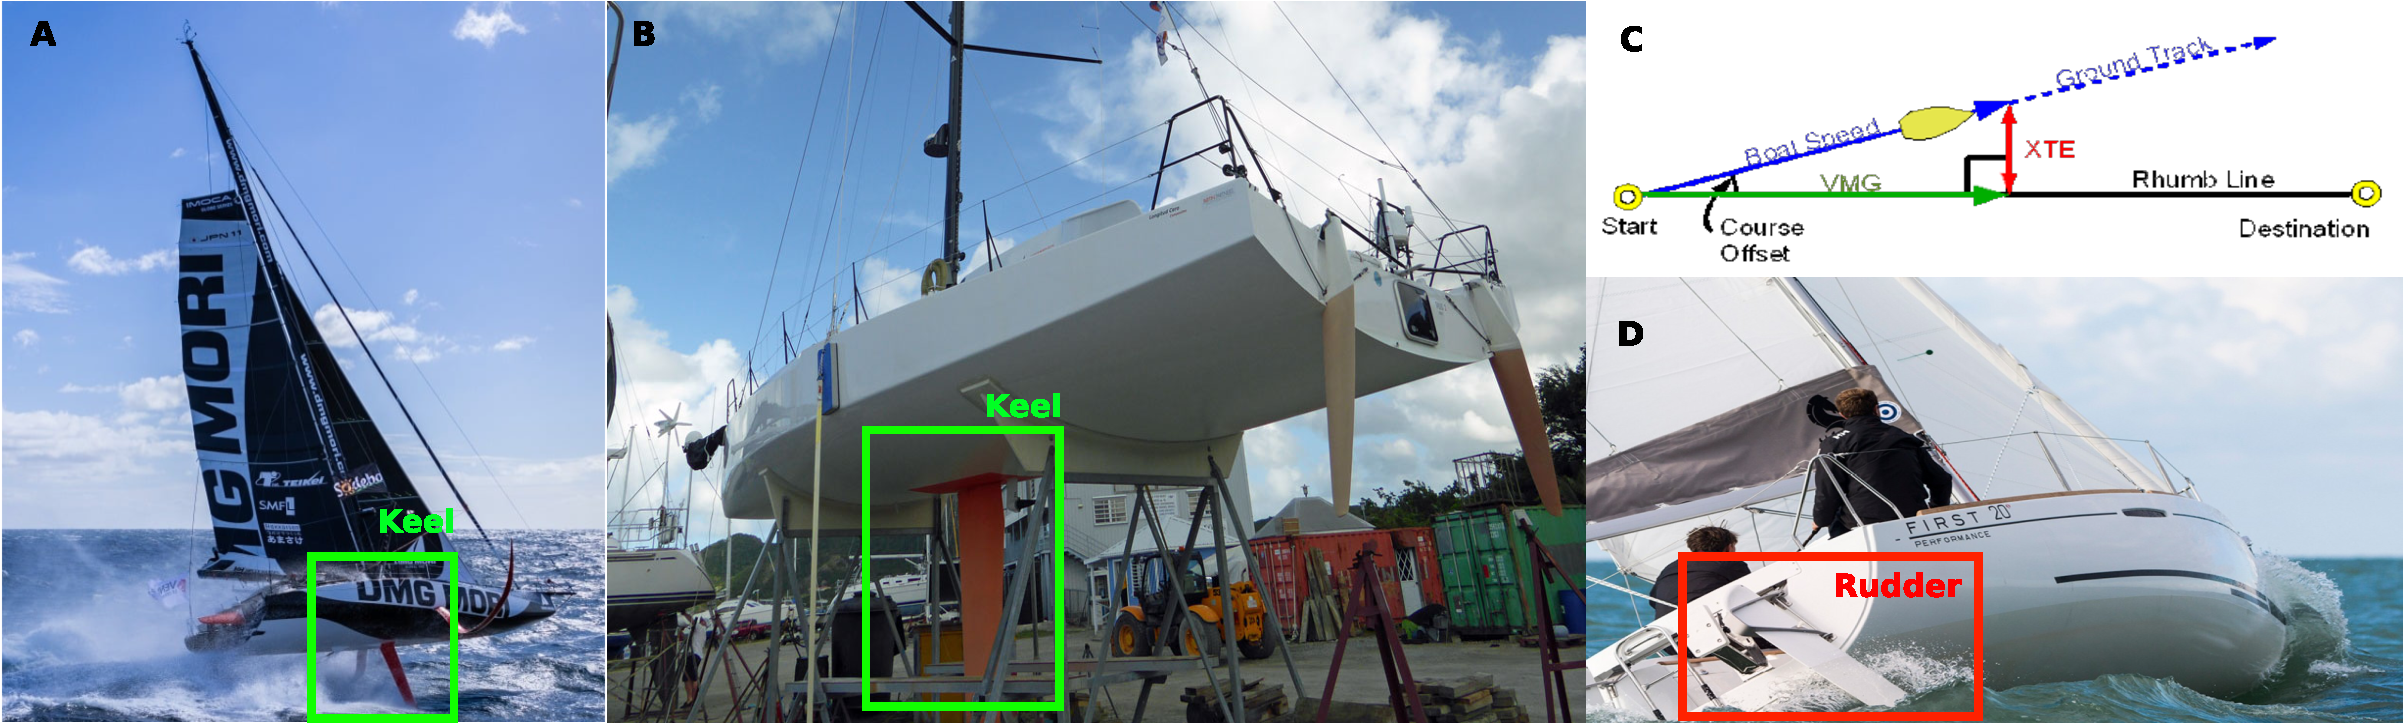
\includegraphics[width=1\linewidth]{resources/img/chapter1/boats_keel.pdf}
    \caption{Sailing dynamics and components of a sailboat. (A \& B) showing the keel (green) for lateral stability. 
    (C) Vector diagram of CMG, course offset, and cross-track error (XTE). 
    (D) Stern close-up showing the rudder (red) for steering.}
    \label{fig:boats}
\end{figure}

\justify The motion of a sailboat is governed by a dynamic equilibrium of Newtonian forces and fluid structure interactions. Propulsion is primarily generated through the \textbf{Coandă Effect}, in which airflow sticks to the curvature of the sail and is redirected backward. According to Newton’s Third Law, this deflection produces an equal and opposite reaction force, resulting in a total aerodynamic force. A component of this force provides the forward thrust ($F_{\text{thrust}}$) necessary to accelerate the vessel to a given velocity ($V_{\text{boat}}$). The net acceleration of the boat can be expressed:
\[
F_{\text{net}} = F_{\text{thrust}} - F_{\text{drag}},
\]
\justify where $F_{\text{drag}}$ includes both aerodynamic resistance and hydrodynamic friction. Maintaining directional efficiency requires a precise control: the keel converts lateral wind pressure into forward motion, while the rudder enables steering at the cost of minor “steering drag.” Mastery of this balance between air and water forces is the ultimate challenge that the RL agent must learn to optimize performance. 

\justify Beyond raw acceleration, the efficiency is measured by its progress toward a target destination. This is quantified by the Course Made Good (CMG), which represents the effective velocity projected onto the intended path. Given a course offset angle $\beta$—the angle between the boat’s heading and the target line CMG is defined as:  
\begin{equation}
    \text{CMG} = V_{\text{boat}} \cdot \cos(\beta)
\end{equation}


\justify Simultaneously, the agent must minimize the Cross-Track Error (XTE), the perpendicular distance from the current position to the target trajectory. If $D$ denotes the distance traveled from the starting point, lateral deviation is expressed as:

\begin{equation}
    \text{XTE} = D \cdot \sin(\beta)
\end{equation}

By optimizing $F_{\text{net}}$ to maintain speed while minimizing XTE, the sailors (agent) maximizes CMG along the most direct trajectory, achieving both efficient propulsion and precise navigation.

%%%%%%%%%%%%%%%%%%%%%%%%%%%%%%%%%%%%%%%%%%%%%%%%%%%%%%%%%%%%%%%%

\subsection{Problem Definition and Navigation Challenge} 
The primary objective of this project is to explore how DRL can extend traditional autopilot capabilities beyond simple set point maintenance, evolving them into intelligent systems capable of strategic navigation under uncertainty.

\subsubsection{Simulation Environment: \emph{BoatSimulator}} 
This study employs a high fidelity Python-based simulation environment called \emph{BoatSimulator}\footnote{Developed at Nautia}, built using the OpenAI Gymnasium framework to model boat dynamics in open sea conditions. For RL compatibility, the simulator is packaged within \emph{boatsgym}, a wrapper compliant with the Gymnasium API. The graphical user interface (GUI) and 3D visualization of the BoatSimulator are presented in Figure \ref{fig:simg}. 

\begin{figure}[H]
    \centering
    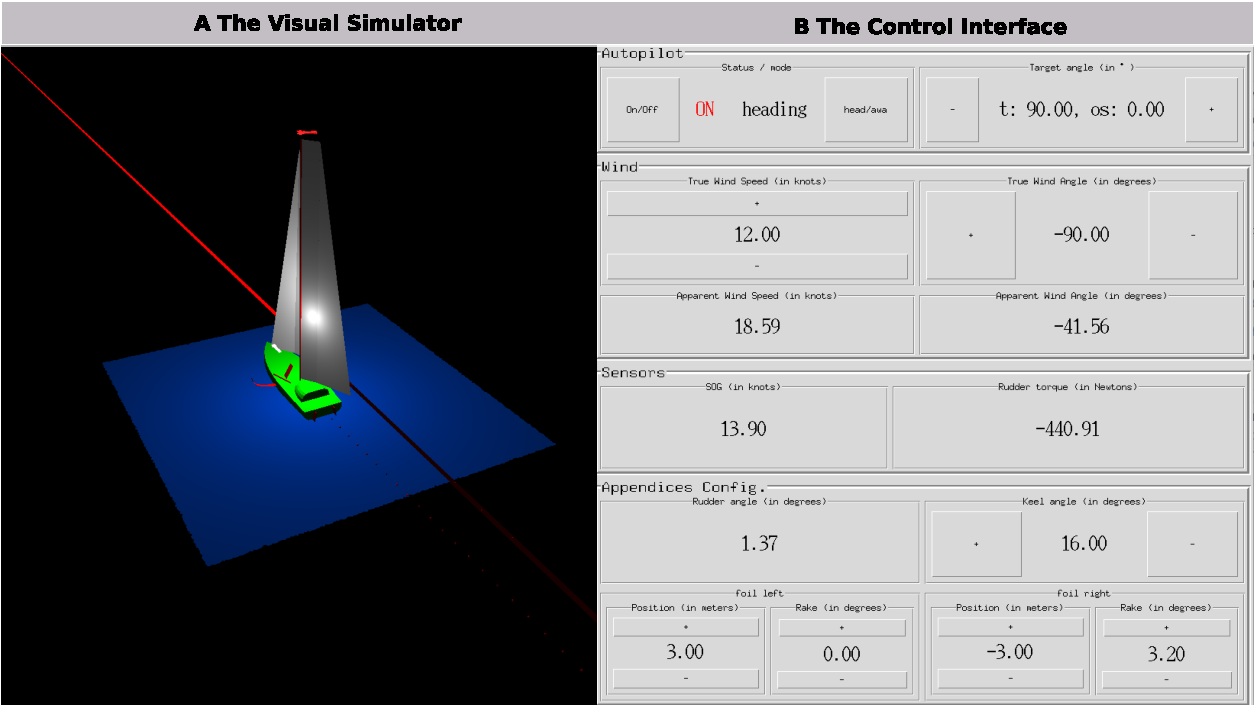
\includegraphics[width=1\linewidth]{resources/img/chapter1/simulator.pdf}
    \caption{The \emph{BoatSimulator} interface, featuring the system control dashboard (left) and 3D environmental viewport (right).}
    \label{fig:simg}
\end{figure}

At the core of the navigation logic in the BoatSimulator is a classical Proportional-Integral-Derivative (PID) control loop which serves as the baseline for this study.

\subsubsection{Baseline PID Performance and Navigation Limitations}

Figure \ref{fig:traje} illustrates a scenario in which the BoatSimulator's PID controller attempts to maintain a target heading of $90^\circ$ under a 12 kt wind. While the controller successfully stabilizes the boat's orientation, a persistent lateral deviation (called leeway) remains. This Cross-Track Error (XTE), visualized as the vertical red lines between the observed path and the target trajectory, arises because the PID controller only regulates angular heading and lacks awareness of the boat’s global position and effective forward progress. As a result although the heading is maintained, the sailboat drifts sideways relative to the intended trajectory, limiting its CMG. 

\begin{figure}[H] 
    \centering 
    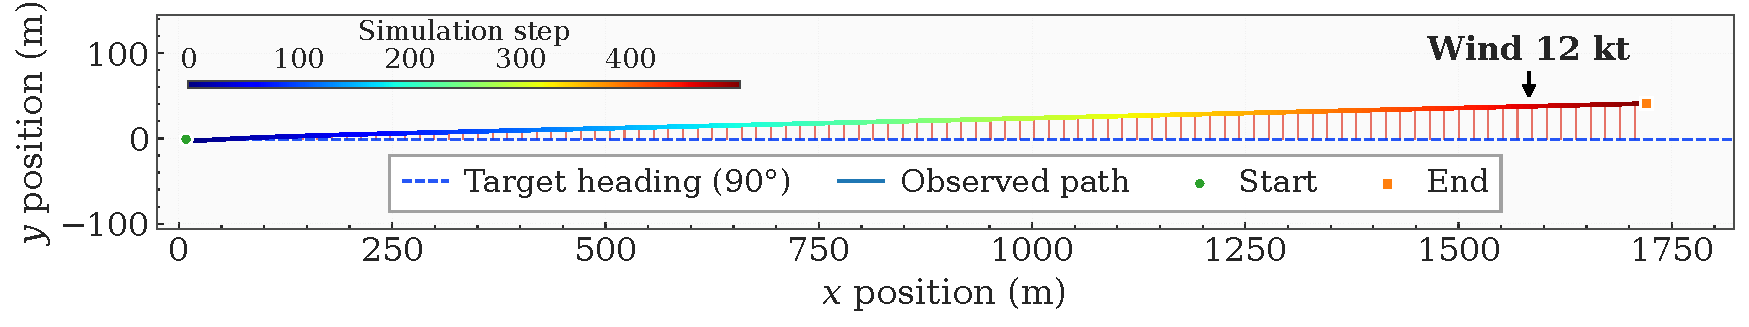
\includegraphics[width=1\linewidth]{resources/img/chapter1/trajectory_xte_pub.pdf} 
    \caption{Trajectory toward $90^\circ$ under 12 kt wind. The blue dashed line represents the target trajectory, while the vertical red lines indicate the accumulation of XTE despite stable heading control.} 
    \label{fig:traje}
\end{figure}

The performance implications of the PID controller’s limitations are further illustrated in Figure \ref{fig:pid-performance}. The CMG reward representing the component of the boat’s velocity aligned with the target trajectory initially spikes as the vessel accelerates but ultimately stabilizes at a sub-optimal mean of $13.89\,\text{m/s}$. Corresponding control plots indicate that the heading error converges to a small non zero value, while the rudder angle stabilizes near $80^\circ$ to counteract wind forces. Despite these stabilizations, the system fails to maximize forward velocity toward the goal.

\begin{figure}[H] 
    \centering 
    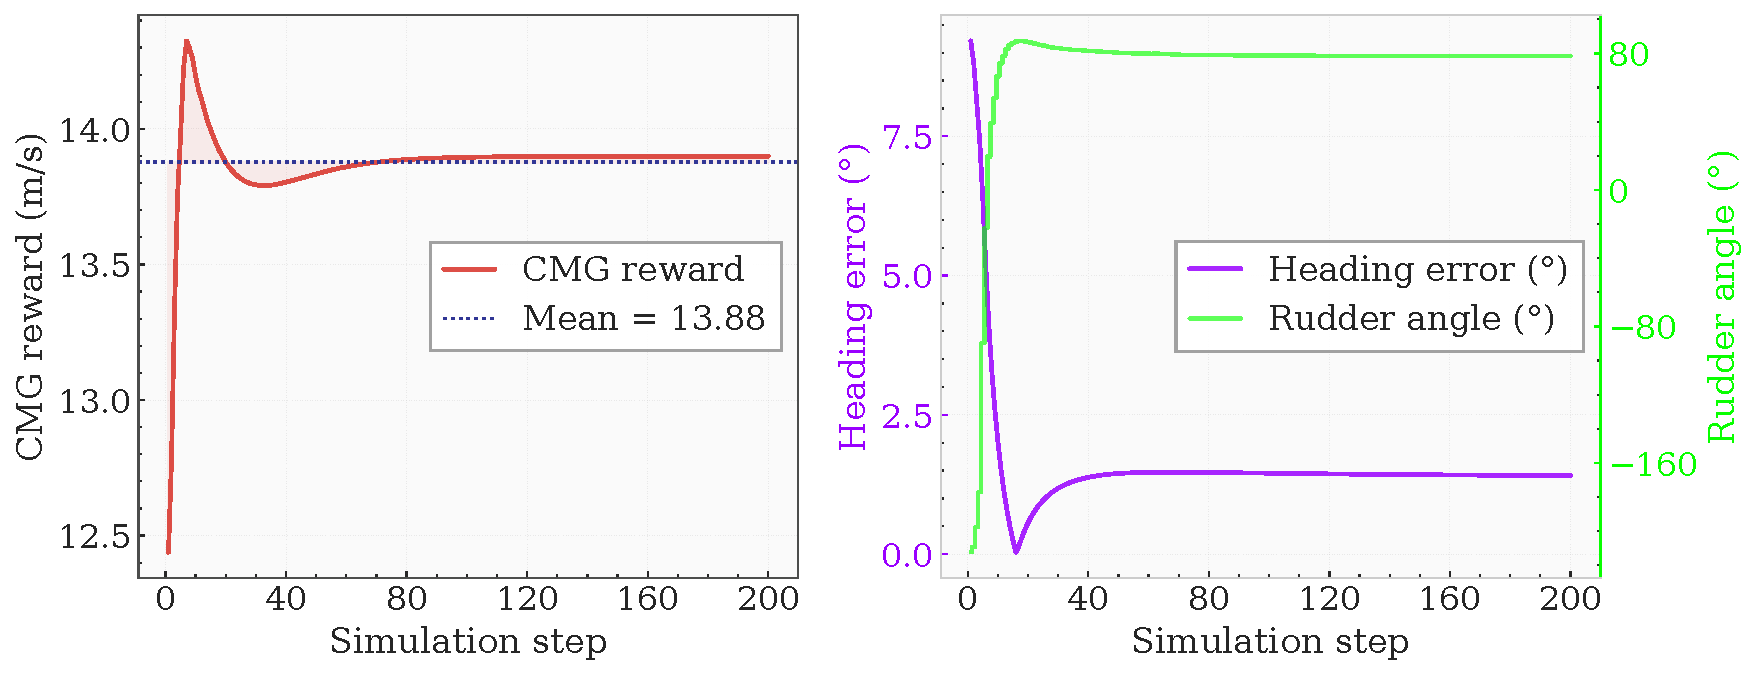
\includegraphics[width=1\linewidth]{resources/img/chapter1/cmg_control_first200_pub.pdf} 
    \caption{Baseline PID performance metrics. \textbf{Left:} CMG reward over time. \textbf{Right:} Heading error and rudder angle stabilization under constant environmental forcing.} 
    \label{fig:pid-performance} 
\end{figure}

Maintaining a constant heading alone is insufficient for maximizing forward progress (CMG). To address this limitation of classical closed-loop controllers, a DRL agent must learn to combine precise heading control with a strategy that proactively maximizes CMG, adapting continuously to stochastic environmental forces and moving beyond the constraints of simple set point regulation.